\begin{enumerate}
  \item 
  \begin{enumerate}
    \item Il suffit de montrer que $f_{1}$ admet en 0 des limites {\`a} droite et {\`a} gauche {\'e}gales. 
\begin{displaymath}
f_{1}(x)=e^{\frac{1}{x}\ln (x+\sqrt{x^{2}+1})}  
\end{displaymath}
Calculons la limite {\`a} droite en 0 en utilisant un développement limité.
\begin{displaymath}
  x+\sqrt{x^{2}+1} = \sqrt{1+x^{2}} + x = 1 + x + o(x) \Rightarrow \frac{1}{x}\ln (x+\sqrt{x^{2}+1})\rightarrow 1
  \Rightarrow f_{1}(x)\rightarrow e
\end{displaymath}
Le calcul pr{\'e}c{\'e}dent est encore valable {\`a} gauche. On prolonge $f_1$ en $f$ par continuit{\'e} en posant $f(0)=e$ et $f(x)=f_1(x)$ si $x\neq 0$.

  \item La fonction $f$ est paire car
\begin{displaymath}
\forall x\neq 0, \; (x+\sqrt{x^{2}+1})(-x+\sqrt{x^{2}+1})=1 \Rightarrow f(-x) = f(x)  
\end{displaymath}

  \item On utilise une dérivée pour accélérer le calcul du d{\'e}veloppement limit{\'e} en 0.
\begin{multline*}
  \left( \ln(x+\sqrt{x^{2}+1})\right)' = \frac{1}{\sqrt{1+x^2}} =  \left( 1+x^2\right)^{-\frac{1}{2}}
  = 1-\frac{1}{2}x^2 + \frac{3}{8}x^4 +o(x^5) \\
  \Rightarrow \ln (x+\sqrt{x^{2}+1}) = x-\frac{1}{6}x^{3}+\frac{3}{40}x^{5}+o\left(x^{6}\right)  \\
\Rightarrow \frac{1}{x}\ln (x+\sqrt{x^{2}+1}) = 1-\frac{1}{6}x^{2}+\frac{3}{40}x^{4}+o\left( x^{5}\right)
\end{multline*}
Soit $f(x)=ee^{v}$, avec $v = -\frac{1}{6}x^{2}+\frac{3}{40}x^{4}+o\left( x^{5}\right) $. On en déduit
\begin{displaymath}
  f(x) = e^{\frac{1}{x}\ln (x+\sqrt{x^{2}+1})} = e  -\frac{e}{6} x^{2} + \frac{4e}{45} x^{4}+o\left( x^{4}\right) \text{ avec }\frac{3}{40} + \frac{1}{2\times 6^2} = \frac{4}{45}.
\end{displaymath}

  \item Calcul de la dérivée de $f$ factorisée par commodité.
\begin{displaymath}
\forall x\neq 0,\; f'(x) = \varphi(x) \frac{f(x)}{x^2} \text{ avec } 
\varphi(x) = \frac{x}{\sqrt{1+x^2}} - \ln\left( x+\sqrt{1+x^2}\right)   
\end{displaymath}
On remarque que $\varphi(0)=0$, on étudie le signe de $\varphi$ (aussi celui de $f'$) en dérivant
\begin{displaymath}
  \varphi'(x) = -\frac{x^2}{(1+x^2)^{\frac{3}{2}}} < 0 .
\end{displaymath}
On en déduit le tableau des signes et des variations
\begin{center}
\begin{tabular}{c|ccc||ccc}
           & $-\infty$ &            & $0_-$& $0_+$ &            & $+\infty$ \\ \hline
 $\varphi'$&           & $-$        &      &       & $-$        & \\ \hline
 $\varphi$ &           & $\searrow$ & $0$  & $0$   & $\searrow$ & \\ \hline
 $\varphi$ &           & $+$        & $0$  & $0$   & $-$        & \\ \hline
 $f$       &           & $\nearrow$ &      &       & $\searrow$ & 
\end{tabular}
\end{center}
\'Etude des limites de $f'$ en $0$ et en $+\infty$.\newline
En $0$, la fonction $f$ est dérivable avec $f'(0) = 0$ qui sur le lit d'après c. sur son développement tronqué à l'ordre 1. Si on était assuré du caractère $\mathcal{C}^1$, on pourrait affirmer sans calcul que la limite de $f'$ en $0$ est $0$. Mais nous n'avons même pas montré la continuité de la dérivée en $0$. Pour justifier cette limite, nous devons reprendre des développements limités en $0$
\begin{displaymath}
\left. 
\begin{aligned}
\frac{\ln\left( x + \sqrt{1+x^2}\right)}{x^2} &= \frac{1}{x} - \frac{x}{6} + o(x^2) \\
\frac{1}{x\sqrt{1+x^2}} &= \frac{1}{x} - \frac{x}{2} + o(x^2)
\end{aligned}
\right\rbrace \Rightarrow 
f'(x) = \left( -\frac{x}{3} + o(x^2)\right)f(x) \rightarrow 0. 
\end{displaymath}
\'Ecrivons des développements en $+\infty$
\begin{multline*}
\sqrt{1+x^2} =x\sqrt{1+\frac{1}{x^2}} = x+\frac{1}{2x} + o(\frac{1}{x})\\
\Rightarrow
\ln\left( \sqrt{1+x^2}+x\right) = \ln\left( 2x+\frac{1}{2x} + o(\frac{1}{x})\right)
= \ln x + \ln 2 + \frac{1}{4x^2} + o(\frac{1}{x^2)}\\
\Rightarrow
\frac{\ln\left( x+\sqrt{1+x^2}\right)}{x} 
= \frac{\ln x}{ x} + O(1)
\end{multline*}
On en déduit que $f \rightarrow 1$ en $+\infty$. D'autre part
\begin{displaymath}
  \frac{x}{\sqrt{1+x^2}} \rightarrow 1 \Rightarrow \varphi(x) \sim - \ln x
  \Rightarrow f'(x) \sim \frac{-\ln x}{ x^2} \rightarrow 0
\end{displaymath}

  
\begin{figure}[h]
  \centering
  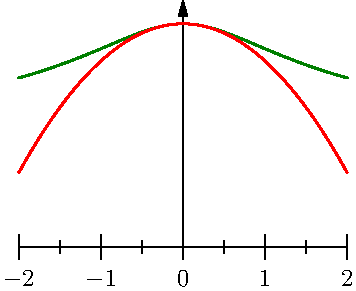
\includegraphics[width=5cm]{./Ccalloc1_1.pdf}
  % Ccalloc1_1.pdf: 0x0 pixel, -2147483648dpi, 0.00x0.00 cm, bb=
  \caption{Graphe de $f$}
  \label{fig:Ccalloc_1}
\end{figure}

  \item On trace {\`a} la machine le graphe de la fonction $f$.  D'apr{\`e}s le d{\'e}veloppement limit{\'e} en $0$,
\begin{displaymath}
  f(x)-e(1-\frac{x^{2}}{6}) = \frac{4e}{45} x^{4} + o\left( x^{4}\right).
\end{displaymath}
Cette expression est positive au voisinage de 0, la courbe est au dessus de la parabole.
  \end{enumerate}

  \item
  \begin{enumerate}
    \item La d{\'e}rivabilit{\'e} de $F$ en 0 (avec $F'(0)=f(0)$) assure la continuit{\'e} de $H $.

    \item La fonction $H$ est deux fois d{\'e}rivable dans $\R_{+}^{*}$ par les opérations habituelles.\newline 
Pour montrer la dérivabilité en $0$ et la valeur de la dérivée, on forme un développement limité à l'ordre $1$ de $H$. Intégrons le d{\'e}veloppement limit{\'e} de $f$ :
\begin{multline*}
f(x)=e-\frac{e}{6}x^{2}+o(x^{2}) \Rightarrow F(x)=ex-\frac{e}{18}x^{3}+o(x^{3})\\
\Rightarrow H(x) = e -\frac{e}{18}x^{2}+o(x^{2})
\Rightarrow H^{\prime }(0)=0
\end{multline*}
Formons un développement de $H'$, pour $x>0$,
\begin{multline*}
\left. 
\begin{aligned}
  \frac{f(x)}{x} =& \frac{e}{x} - \frac{e}{6}x +o(x) \\
  \frac{F(x)}{x^2} =& \frac{e}{x} - \frac{e}{18}x +o(x)
\end{aligned}
\right\rbrace 
\Rightarrow
 H^{\prime }(x)=\frac{f(x)}{x}-\frac{F(x)}{x^{2}} = -\frac{e}{9}x + o(x) \\
 \Rightarrow H''(0)=-\frac{e}{9}.
\end{multline*}

\begin{multline*}
 H^{\prime }(x)=\frac{f(x)}{x}-\frac{F(x)}{x^{2}} 
 \Rightarrow \frac{H^{\prime }(x)-H^{\prime }(0)}{x}
 =\frac{xf(x)-F(x)}{x^{3}}
 =(-\frac{e}{6}+\frac{e}{18})+o(1) \\
 \Rightarrow H''(0) = -\frac{e}{9}.
\end{multline*}

     \item Pour $x>0$, consid{\'e}rons la fonction $t\rightarrow F(t)-tf(x)$ dans $\left[ 0,x\right]$.\newline
     Sa d{\'e}riv{\'e}e $f(t)-f(x)$ est positive car $f$ est décroissante dans $[0+\infty[$. On en d{\'e}duit en particulier que $F(x)\geq xf(x)$ d'o{\`u} $H(x)\geq f(x)$.

     \item Au voisinage de $+\infty $, on peut {\'e}crire :
\[
\frac{1}{x}\ln \left( x+\sqrt{x^{2}+1}\right) =\frac{1}{x}\left[ \ln x+%
\underset{\longrightarrow \ln 2}{\ln \left( 1+\sqrt{1+\frac{1}{x^{2}}}%
\right) }\right] \sim \frac{\ln x}{x}\rightarrow 0 .
\]
On en d{\'e}duit que $f$ tend vers 1 avec $f(x)-1\sim \frac{\ln x}{x}$.\newline
Consid{\'e}rons $g(x)=F(x)-x-2\sqrt{x}$.\newline
Alors $g^{\prime }(x)=f(x)-1-\frac{1}{\sqrt{x}}\sim -\frac{1}{\sqrt{x}}$ car $\frac{\ln x}{x}$ est négligeable en $+\infty$ devant $\frac{1}{\sqrt{x}}$.\newline
Il existe donc un $x_{0}>0$ tel que $g$ soit strictement d{\'e}croissante dans $\left[x_{0},+\infty \right[ $.\newline
On en d{\'e}duit $F(x)\leq g(x_{0})+x+2\sqrt{x}$ pour tout $x\geq x_{0}$ puis
\[
f(x)\leq H(x)\leq \frac{g(x_{0})}{x}+1+\frac{2}{\sqrt{x}}\text{.}
\]
Ce qui montre, avec le th{\'e}or{\`e}me d'encadrement, que $H(x)$ tend vers 1 en $+\infty $.
  \end{enumerate}

  \item 
  \begin{enumerate}
    \item La fonction $F$ est strictement croissante dans $\R_{+}$. D'apr{\`e}s 2.c.,
\begin{displaymath}
F(x)\geq xf(x)\geq x \Rightarrow F(x) \xrightarrow{+\infty} +\infty .
\end{displaymath}
Comme $F$ est continue, $F(\R_{+})=\R_{+}$. Elle est bijective vers son image. Elle admet une bijection r{\'e}ciproque $G$ continue strictement croissante de $\R_{+}$ dans $\R_{+}$.

    \item Comme $F^{\prime }(x)=f(x)>0$ pour tous les $x$ positifs, le théorème de la dérivabilité de la bijection réciproque assure que $G$ est dérivable avec
\[
\forall t\geq 0,\; G^{\prime }(t)=\frac{1}{F^{\prime }(G(t))}=\frac{1}{f(G(t))}.
\]
Remarquons que $G(0)=0$ car $F(0)=0$ et appliquons le th{\'e}or{\`e}me des accroissements finis {\`a} $G$ dans $\left[ 0,u\right] $. Il existe $c\in \left] 0,u\right[ $ tel que $G(u)-G(0) = uG^{\prime }(c) = \frac{u}{f(v)}$ en posant $v=G(c)$. Comme $G$ est d{\'e}croissante, $v\in \left] 0,G(u)\right[ $ et v{\'e}rifie la formule de l'{\'e}nonc{\'e}.
  \end{enumerate}
\end{enumerate}

